\documentclass[12pt,a4paper]{article}

\usepackage[utf8]{inputenc}
\usepackage[T1]{fontenc}
\usepackage[brazil]{babel}
\usepackage{geometry}
\geometry{a4paper, margin=2.5cm}
\usepackage{graphicx}
\usepackage{xurl}
\usepackage{hyperref}
\usepackage{listings}
\usepackage{xcolor}

% Configuracao para exibicao de blocos de codigo e comandos
\lstset{
    basicstyle=\ttfamily\footnotesize,
    backgroundcolor=\color{gray!10},
    frame=single,
    breaklines=true,
    captionpos=b,
    showstringspaces=false
}

\begin{document}

% ================= CAPA =================
\begin{titlepage}
    \centering
    \vspace*{4cm}

    {\Huge \bfseries Relatório Final: Laboratórios de Redes de Computadores\par}
    \vspace{1.5cm}
    {\Large \bfseries Mininet e Ryu + OpenFlow\par}

    \vspace{4cm}
    {\Large Autor: Uálaci dos Anjos Júnior\par}

    \vfill
    {\large \today\par}
\end{titlepage}

% ================= CONTEÚDO =================

\section{Introdução e Configuração do Ambiente}

\textbf{Repositório Base em Nuvem:} \url{https://github.com/ualaci/report2-mininet-ryu-ppcomp-mpca-comp-networks}

Este documento descreve os testes e os resultados dos laboratórios 1 (Mininet) e 2 (Ryu + OpenFlow). O objetivo principal foi aplicar na prática os conceitos de Redes Definidas por Software (SDN), observando a comunicação entre a rede emulada pelo Mininet e o controlador Ryu. O texto foca em explicar a parte técnica de forma simples e direta.

O ambiente de testes usou o sistema Ubuntu 20.04. Foram instaladas ferramentas como Open vSwitch, Mininet 2.3 e Wireshark.
Logo no primeiro teste usando o comando básico do emulador (\texttt{sudo mn}), o sistema mostrou um erro indicando que faltava um controlador:

\begin{lstlisting}
*** No default OpenFlow controller found for default switch!
*** Falling back to OVS Bridge
\end{lstlisting}

Esse erro acontece porque o pacote \texttt{openvswitch-testcontroller} não existe mais nas versões novas do Ubuntu. Sem um controlador conectado na porta padrão de SDN, o Open vSwitch (OVS) entra em um modo de segurança (\textit{fallback}). Nesse modo, ele passa a funcionar como um switch comum da camada 2 (apenas encaminhando endereços MAC), mas sem usar o protocolo OpenFlow.

Para corrigir isso e fazer o laboratório funcionar como uma rede SDN real, foi usado o controlador externo Ryu. Em todos os testes, o Mininet foi iniciado com a opção \texttt{--controller remote}. Isso fez o switch parar de enviar dados sozinho e esperar as ordens de roteamento da porta 6653, que é onde o programa do Ryu estava rodando.

\section{Laboratório 1: Emulação de Redes com Mininet}

A primeira parte do laboratório consistiu em testar os comandos básicos do Mininet no terminal e, depois, criar scripts em Python para montar uma rede maior e personalizada.

\subsection{Fase 1: Comandos Básicos (Everyday Mininet Usage)}

Os resultados detalhados desta etapa podem ser conferidos no log empírico disponível em: \url{https://github.com/ualaci/report2-mininet-ryu-ppcomp-mpca-comp-networks/blob/main/relatorio_walkthrough.md}.

Nesta etapa, as operações básicas descritas no tutorial oficial do Mininet foram testadas.
A topologia inicial foi a do tipo \texttt{minimal}, que tem apenas um switch conectado a dois computadores (hosts). A organização da rede foi verificada usando o próprio terminal do emulador:

\begin{lstlisting}
mininet> nodes
available nodes are: 
c0 h1 h2 s1

mininet> dump
<Host h1: h1-eth0:10.0.0.1 pid=11273> 
<Host h2: h2-eth0:10.0.0.2 pid=11275> 
<OVSSwitch s1: lo:127.0.0.1,s1-eth1:None,s1-eth2:None pid=11280> 
<RemoteController c0: 127.0.0.1:6653 pid=11254> 
\end{lstlisting}

O recurso que separa as redes no Linux (chamado de \textit{network namespaces}) foi testado executando o comando \texttt{ifconfig -a} dentro do host emulado h1. O resultado mostrou que a placa de rede virtual tem endereços de IP isolados e não afeta o computador físico:

\begin{lstlisting}
mininet> h1 ifconfig -a
h1-eth0: flags=4163<UP,BROADCAST,RUNNING,MULTICAST>  mtu 1500
        inet 10.0.0.1  netmask 255.0.0.0  broadcast 10.255.255.255
...
\end{lstlisting}

A comunicação da rede foi confirmada com o comando \texttt{pingall}, que testou o alcance entre todas as máquinas com 100\% de sucesso.

\subsection{Fase 1: Inicialização Avançada}

Os testes de inicialização parametrizada descritos a seguir baseiam-se nos logs evidenciados em: \url{https://github.com/ualaci/report2-mininet-ryu-ppcomp-mpca-comp-networks/blob/main/relatorio_full_walkthrough.md}.

Foram feitos testes passando opções extras na hora de iniciar o Mininet. O teste de velocidade da rede usando o programa Iperf mostrou a capacidade máxima do sistema:

\begin{lstlisting}
$ sudo mn --test iperf --controller remote
*** Iperf: testing TCP bandwidth between h1 and h2 
*** Results: ['32.1 Gbits/sec', '32.2 Gbits/sec']
\end{lstlisting}
Esse resultado alto (acima de 30 Gbits/sec) mostra que a rede virtual do Mininet roda de forma muito rápida quando não há limites configurados.

O formato da rede também foi alterado pelo parâmetro \texttt{--topo}. O formato em linha (onde vários switches ficam ligados em sequência) funcionou perfeitamente:

\begin{lstlisting}
$ sudo mn --test pingall --topo linear,4 --controller remote
*** Ping: testing ping reachability
h1 -> h2 h3 h4 
h2 -> h1 h3 h4 
...
*** Results: 0% dropped (12/12 received)
\end{lstlisting}

Para simular problemas do mundo real, usou-se a opção \texttt{TCLink}. Isso limitou a velocidade dos cabos virtuais para 10 Mbps e adicionou um atraso de 10 milissegundos:

\begin{lstlisting}
$ sudo mn --link tc,bw=10,delay=10ms --test iperf --controller remote
*** Iperf: testing TCP bandwidth between h1 and h2 
*** Results: ['9.50 Mbits/sec', '12.0 Mbits/sec']
\end{lstlisting}
A medição mostrou que a rede obedeceu corretamente aos limites definidos.

\subsection{Fase 1: Manipulação da API na Linha de Comando}

O terminal do Mininet permite alterar os cabos virtuais enquanto a rede está ligada. Foi feito um teste derrubando o cabo de rede para ver a reação do sistema:

\begin{lstlisting}
mininet> link s1 h1 down
mininet> pingall
*** Results: 100% dropped (0/2 received)

mininet> link s1 h1 up
mininet> pingall
*** Results: 0% dropped (2/2 received)
\end{lstlisting}
Quando a conexão foi religada (\texttt{link up}), os testes de Ping voltaram a funcionar, provando que é possível simular falhas físicas no software.

\subsection{Fase 2: Topologia Customizada em Python}

O desenvolvimento da topologia dinâmica via script abordada a seguir foi baseado no código e logs disponíveis em: \url{https://github.com/ualaci/report2-mininet-ryu-ppcomp-mpca-comp-networks/blob/main/relatorio_phase2.md} e no script \texttt{lab1\_phase2.py}.

Em vez de digitar os comandos um a um, o laboratório exigiu o uso de um script em Python para criar a rede de forma automática.

Para criar 4 switches e 11 hosts, foi programada a classe \texttt{CustomTopo}. No código, os switches de \texttt{s1} a \texttt{s4} foram criados e conectados em fila:
\begin{lstlisting}[language=Python]
self.addLink( s1, s2 )
self.addLink( s2, s3 )
self.addLink( s3, s4 )
\end{lstlisting}

Um laço de repetição (loop) criou os hosts \texttt{h1} a \texttt{h11}. Eles foram divididos entre os switches, e todos os cabos foram configurados com limites muito rígidos: 10 Mbps de banda, 5ms de atraso e 2\% de perda forçada de pacotes:
\begin{lstlisting}[language=Python]
self.addLink( h, s1, bw=10, delay='5ms', loss=2, max_queue_size=1000, use_htb=True )
\end{lstlisting}

Uma função customizada de teste (\texttt{perfTest}) foi criada para fazer o host principal (\texttt{h1}) mandar um teste de Iperf para todos os outros hosts de forma automática.
Devido à regra de 2\% de perda imposta nos cabos, o teste global de Ping falhou de propósito em 9\% das tentativas:
\begin{lstlisting}
*** Ping: testing ping reachability
*** Results: 9% dropped (100/110 received)
\end{lstlisting}
Isso provou que o código aplicou com sucesso as restrições de uma rede congestionada.

\begin{figure}[htbp]
    \centering
    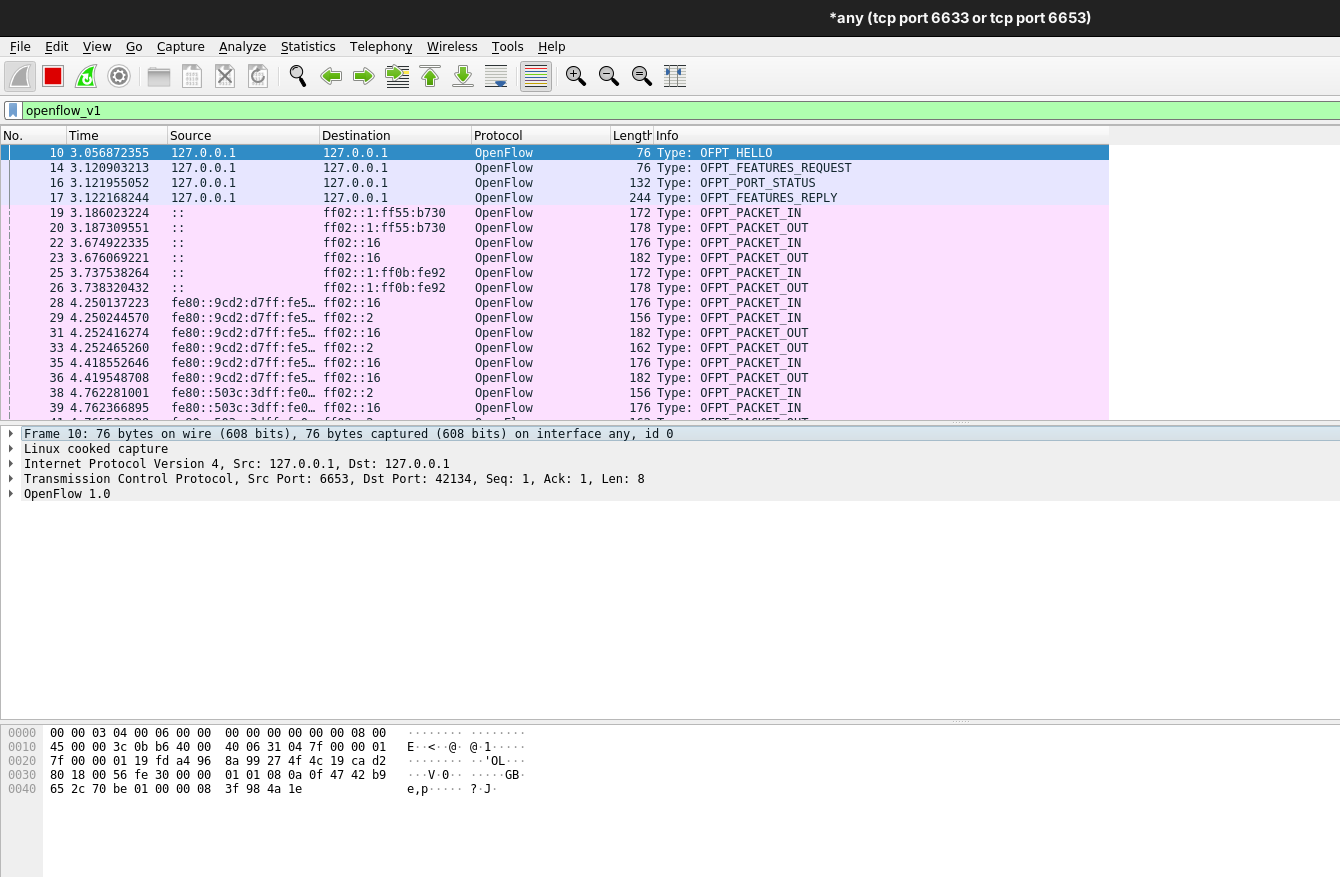
\includegraphics[width=0.9\textwidth]{lab1_images/openflow simple switch.png}
    \caption{Captura e análise do fluxo de mensagens no Laboratório 1}
    \label{fig:lab1_openflow}
\end{figure}

\section{Laboratório 2: SDN com Controlador Ryu e OpenFlow}

Na segunda etapa, o foco mudou para a análise do protocolo OpenFlow 1.3, capturando e entendendo as mensagens trocadas entre o Ryu e o switch.

\subsection{Iniciando a Rede SDN}

A rede foi iniciada com o seguinte comando simples:
\begin{lstlisting}
sudo mn --topo single,3 --mac --controller remote --switch ovsk,protocols=OpenFlow13
\end{lstlisting}
O parâmetro \texttt{--mac} definiu endereços fáceis de ler (como \texttt{00:00:00:00:00:01} para o h1), ajudando muito a não se perder na análise feita dentro do Wireshark.

\subsection{Comportamento do Switch sem Controlador}

Com o Wireshark aberto gravando a rede, tentou-se mandar um Ping sem ligar o controlador Ryu no terminal.

\begin{lstlisting}
mininet> h1 ping -c 1 h2
PING 10.0.0.2 (10.0.0.2) 56(84) bytes of data.
--- 10.0.0.2 ping statistics ---
1 packets transmitted, 0 received, 100% packet loss, time 0ms
\end{lstlisting}

Isso aconteceu porque, no modo OpenFlow, o switch "esquece" como funciona a rede tradicional. Ele não sabe o que fazer com os pacotes e, como o Ryu estava desligado para instruí-lo, o switch simplesmente bloqueou e destruiu a comunicação.

\subsection{Conexão e Negociação (Handshake)}

Em seguida, o controlador foi ativado no terminal:
\begin{lstlisting}
$ ryu-manager ryu.app.simple_switch_13
\end{lstlisting}

Logo que o Ryu iniciou, o Wireshark mostrou uma série de mensagens. Essa é a negociação padrão do OpenFlow:
\begin{enumerate}
    \item \textbf{HELLO:} O switch e o controlador avisam que vão usar a versão 1.3 do protocolo.
    \item \textbf{FEATURES\_REQUEST e REPLY:} O controlador pergunta as configurações do switch, e o switch responde enviando seu número de identificação e a quantidade de tabelas que possui.
    \item \textbf{Criação da Regra Padrão (Table-Miss):} Essa é a parte mais importante. O Ryu manda uma mensagem chamada \texttt{FLOW\_MOD} criando uma regra de prioridade zero (a mais baixa). Essa regra diz ao switch: "Se chegar um pacote que você não conhece, não apague. Envie ele todo para mim."
\end{enumerate}

\subsection{O Comportamento do Learning Switch}

Com a regra principal criada, repetiu-se o teste de Ping:
\begin{lstlisting}
mininet> h1 ping -c 1 h2
64 bytes from 10.0.0.2: icmp_seq=1 ttl=64 time=3.91 ms
\end{lstlisting}
Desta vez, funcionou. O passo a passo registrado no Wireshark foi:
\begin{enumerate}
    \item O host h1 enviou a pergunta (ARP) procurando o host h2. O switch não sabia o caminho e enviou o pacote para o controlador (mensagem \texttt{PACKET\_IN}).
    \item O controlador aprendeu que a máquina h1 estava conectada na porta 1.
    \item Como não sabia onde h2 estava, o controlador ordenou que o switch encaminhasse o pacote para todas as portas ativas (inundação).
    \item O host h2 respondeu. O pacote passou de novo para o controlador, que aprendeu que h2 estava na porta 2.
    \item Agora conhecendo todo o caminho, o controlador enviou ordens definitivas ao switch (\texttt{FLOW\_MOD}). Ele criou regras dizendo: "Pacotes para h2 vão pela porta 2. Pacotes para h1 vão pela porta 1".
\end{enumerate}

\begin{figure}[htbp]
    \centering
    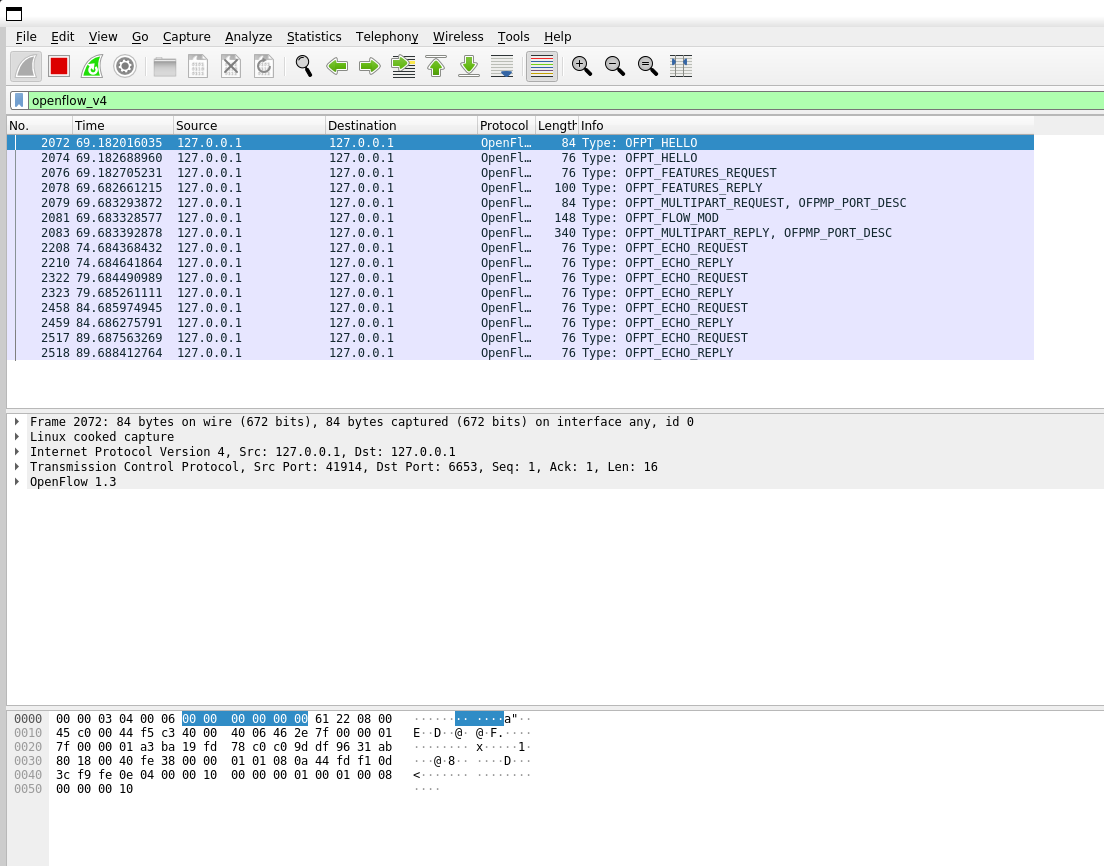
\includegraphics[width=0.9\textwidth]{lab2_images/Screenshot_2.png}
    \caption{Captura de pacotes e fluxo de mensagens OpenFlow no Laboratório 2}
    \label{fig:lab2_openflow}
\end{figure}

\subsection{Tabelas de Fluxo}

Para checar se o controlador realmente ensinou o switch, foi executado o comando para ler a memória do switch:

\begin{lstlisting}
$ sudo ovs-ofctl dump-flows s1 -O OpenFlow13

 cookie=0x0, duration=15.1s, table=0, n_packets=4, n_bytes=340, priority=0 actions=CONTROLLER:65535
 cookie=0x0, duration=3.5s, table=0, n_packets=2, n_bytes=196, priority=1,in_port=1,dl_dst=00:00:00:00:00:02,dl_src=00:00:00:00:00:01 actions=output:2
 cookie=0x0, duration=3.5s, table=0, n_packets=1, n_bytes=98, priority=1,in_port=2,dl_dst=00:00:00:00:00:01,dl_src=00:00:00:00:00:02 actions=output:1
\end{lstlisting}

A leitura mostrou três coisas:
\begin{enumerate}
    \item A regra de segurança (\textit{Table-Miss}) com prioridade 0 enviando coisas desconhecidas para o controlador.
    \item Uma regra com prioridade 1 enviando pacotes da porta 1 para a porta 2.
    \item Uma regra de volta com prioridade 1 enviando pacotes da porta 2 para a porta 1.
\end{enumerate}
Depois que essas regras foram gravadas, o controlador parou de trabalhar no processo de Ping entre essas duas máquinas. O switch começou a encaminhar os pacotes de forma autônoma e rápida pelo hardware.

\section{Conclusão}

Os dois laboratórios cumpriram o objetivo de mostrar como uma rede baseada em SDN funciona na prática. No primeiro laboratório, o Mininet provou ser uma ferramenta muito realista, pois o isolamento do Linux permite criar testes pesados de carga (com latência e perda) em uma rede grande apenas com poucas linhas de código em Python.

No segundo laboratório, ficou clara a separação de papéis na rede. O switch sozinho é incapaz de conectar computadores até que o cérebro central (o Ryu) envie a regra de emergência (\textit{Table-Miss}). O programa transformou uma máquina vazia em um "Switch que Aprende", usando mensagens simples para memorizar portas e depois gravar as rotas no aparelho físico. Isso é ótimo, pois evita que o servidor principal fique sobrecarregado depois que o caminho inicial foi descoberto.

\section{Anexos e Referências de Código}

Todos os artefatos de software desenvolvidos e os logs completos gerados ao longo destes experimentos, bem como os arquivos estáticos de captura do Wireshark (.pcapng), encontram-se disponíveis no repositório vinculado a esta entrega. Abaixo seguem os links para o código em nuvem:

\begin{itemize}
    \item \textbf{Projeto e Documentação Original}: \url{https://github.com/ualaci/report2-mininet-ryu-ppcomp-mpca-comp-networks/blob/main/project_description.txt}
    \item \textbf{Scripts Shell do Lab 2 Ryu}: \url{https://github.com/ualaci/report2-mininet-ryu-ppcomp-mpca-comp-networks/tree/main/scripts}
    \item \textbf{Código Fonte Python da Topologia Custom (Lab 1)}: \url{https://github.com/ualaci/report2-mininet-ryu-ppcomp-mpca-comp-networks/blob/main/scripts/lab1_phase2.py}
    \item \textbf{Logs da Execução - Parte 1 Básica}: \url{https://github.com/ualaci/report2-mininet-ryu-ppcomp-mpca-comp-networks/blob/main/relatorio_walkthrough.md}
    \item \textbf{Logs da Execução - Parte 1 Avançada}: \url{https://github.com/ualaci/report2-mininet-ryu-ppcomp-mpca-comp-networks/blob/main/relatorio_full_walkthrough.md}
    \item \textbf{Logs da Execução - Parte 2 Python Custom}: \url{https://github.com/ualaci/report2-mininet-ryu-ppcomp-mpca-comp-networks/blob/main/relatorio_phase2.md}
\end{itemize}

\end{document}
